% !TEX root = main.tex
\chapter{Metodologi dan Desain Sistem}

Bab ini menguraikan metodologi penelitian, desain arsitektur sistem, dan prosedur eksperimen yang dirancang secara sistematis menggunakan \textit{preprocessing pipeline} terpadu satu jalur untuk mengevaluasi serta membandingkan performa adaptasi \textit{transfer learning} model DINOv3 ViT-L/16 dan ViT-S/16 dalam tugas klasifikasi tingkat keparahan jerawat pada dataset ACNE04.

% -----------------------------------------------------------------------------
\section{Alur Metodologi Penelitian}

Penelitian ini dilaksanakan melalui tahapan eksperimen terstruktur yang mencakup studi literatur, eksplorasi serta \textit{preprocessing} data terstandarisasi, augmentasi klinis dan \textit{fine-tuning} model \textit{transfer learning} DINOv3, hingga pengujian independen dan evaluasi komparatif. Seluruh rangkaian metodologi terbagi ke dalam tiga fase utama yang dilengkapi penandaan blok kontribusi penelitian serta konektor transisi berkonteks (\textbf{A}, \textbf{B}, dan \textbf{C}) sebagaimana diilustrasikan pada diagram alir Gambar~\ref{fig:flowchart_metodologi}.

\begin{figure}[!htbp]
    \centering
    \resizebox{\textwidth}{!}{%
        \begin{tikzpicture}[
                >=Latex,
                font=\sffamily,
                phasehdr/.style={rectangle, rounded corners=2pt, draw=headerblue, fill=headerblue, text=white, minimum width=3.65cm, minimum height=0.62cm, text width=3.55cm, align=center, font=\scriptsize\bfseries},
                startstop/.style={ellipse, draw=black, line width=0.8pt, fill=white, minimum width=2.4cm, minimum height=0.72cm, align=center, font=\footnotesize\bfseries},
                process/.style={rectangle, rounded corners=2pt, draw=black, line width=0.8pt, fill=white, minimum width=3.55cm, minimum height=0.92cm, text width=3.35cm, font=\scriptsize, align=center, inner sep=3.5pt},
                contribdata/.style={rectangle, rounded corners=2.5pt, draw=headerblue, dashed, line width=1.15pt, fill=boxbgblue, minimum width=3.55cm, minimum height=0.98cm, text width=3.35cm, font=\scriptsize, align=center, inner sep=3.5pt},
                contribmodel/.style={rectangle, rounded corners=2.5pt, draw=red!75!black, dashed, line width=1.15pt, fill=red!4, minimum width=3.55cm, minimum height=0.98cm, text width=3.35cm, font=\scriptsize, align=center, inner sep=3.5pt},
                decision/.style={diamond, draw=black, line width=0.8pt, fill=white, aspect=2.0, text width=2.35cm, font=\scriptsize, inner sep=1pt, align=center},
                connector/.style={circle, draw=headerblue, line width=0.9pt, fill=boxbgblue, minimum size=0.68cm, font=\footnotesize\bfseries, text=headerblue},
                connlbl/.style={font=\tiny, text=gray!70!black, align=left, inner sep=1pt},
                arr/.style={thick, ->, draw=black!85}
            ]

            % ==================== KOLOM 1 (X = 0): FASE I ====================
            \node (hdr1) [phasehdr] at (0, 1.05) {FASE I: DATA \& PREPROCESSING};
            \node (start) [startstop] at (0, 0) {Mulai};
            \node (lit) [process, below=0.45cm of start] {Studi Literatur\\(Hayashi, ViT, \& DINOv3)};
            \node (data) [process, below=0.45cm of lit] {Akuisisi Dataset ACNE04\\($1.457$ Citra Klinis)};
            \node (eda) [process, below=0.45cm of data] {\textit{Exploratory Data}\\ \textit{Analysis} (EDA)\\(Rasio 4,91:1 \& $a^*$)};
            \node (prep) [contribdata, below=0.45cm of eda] {\textbf{\textit{Unified Preprocessing}:}\\Face Crop, Skin Mask, Gray World,\\CLAHE, \& Resize $224\times224$};
            \node (split) [process, below=0.45cm of prep] {\textit{Stratified Split} (70:15:15)\\1.019 Train / 219 Val / 219 Test};
            \node (connA1) [connector, below=0.50cm of split] {A};
            \node[connlbl, right=0.18cm of connA1] {\textbf{Konteks A:}\\Data Ter-preprocess \&\\Split Siap Dilatih};

            \draw [arr] (start) -- (lit);
            \draw [arr] (lit) -- (data);
            \draw [arr] (data) -- (eda);
            \draw [arr] (eda) -- (prep);
            \draw [arr] (prep) -- (split);
            \draw [arr] (split) -- (connA1);

            % ==================== KOLOM 2 (X = 7.4): FASE II ====================
            \node (hdr2) [phasehdr] at (7.4, 1.05) {FASE II: AUGMENTASI \& TRAINING};
            \node (connA2) [connector] at (7.4, 0) {A};
            \node[connlbl, right=0.18cm of connA2] {Masuk dari\\Fase I (Split Siap)};
            \node (aug) [contribdata, below=0.45cm of connA2] {\textbf{\textit{Data Augmentation} (Train):}\\H-Flip ($p=0,5$), Safe Rotation\\($\pm 15^\circ$), \& ColorJitter ($\pm 10\%$)};
            \node (train) [contribmodel, below=0.45cm of aug] {\textbf{Komparasi Terkontrol DINOv3:}\\ViT-L/16 (304M) vs ViT-S/16 (21,6M)\\+ \textit{Weighted Cross-Entropy}};
            \node (eval_val) [process, below=0.45cm of train] {Evaluasi Validasi (219 Citra):\\Val Loss \& Val Macro-F1};
            \node (dec1) [decision, below=0.55cm of eval_val] {Model Konvergen\\\& Optimal?};
            \node (impl) [process, below=0.55cm of dec1] {Simpan \textit{Best Checkpoints}\\(Val Macro-F1 Tertinggi)};
            \node (connB1) [connector, below=0.50cm of impl] {B};
            \node[connlbl, right=0.18cm of connB1] {\textbf{Konteks B:}\\\textit{Best Checkpoints}\\Siap Diuji};

            % Tuning node neatly placed in clear gap between Kolom 1 and Kolom 2
            \node (tuning) [process, text width=2.65cm, minimum width=2.80cm, minimum height=0.88cm] at (3.7, -4.85) {\textit{Hyperparameter}\\Tuning\\(LR, WD, Weights)};

            \draw [arr] (connA2) -- (aug);
            \draw [arr] (aug) -- (train);
            \draw [arr] (train) -- (eval_val);
            \draw [arr] (eval_val) -- (dec1);
            \draw [arr] (dec1.west) -| node[pos=0.22, above, font=\tiny, fill=white, inner sep=1pt] {Belum} (tuning.south);
            \draw [arr] (tuning.north) |- (train.west);
            \draw [arr] (dec1.south) -- node[right=2pt, font=\tiny] {Sudah} (impl.north);
            \draw [arr] (impl) -- (connB1);

            % ==================== KOLOM 3 (X = 14.3): FASE III ====================
            \node (hdr3) [phasehdr] at (14.3, 1.05) {FASE III: PENGUJIAN \& EVALUASI};
            \node (connB2) [connector] at (14.3, 0) {B};
            \node[connlbl, right=0.18cm of connB2] {Masuk dari\\Fase II (Checkpoints)};
            \node (gtruth) [process, below=0.45cm of connB2] {\textit{Independent Test Inference}\\(219 Citra Terisolasi)};
            \node (eval_sys) [contribmodel, below=0.45cm of gtruth] {\textbf{Evaluasi Multi-Metrik Klinis:}\\Accuracy, Macro-F1, QWK,\\Class 3 Recall, Matrix 0--3};
            \node (connC1) [connector, below=0.50cm of eval_sys] {C};
            \node[connlbl, right=0.18cm of connC1] {\textbf{Konteks C:}\\Metrik Kuantitatif \&\\Profil Komputasi Siap};
            \node (report) [process, below=0.50cm of connC1] {Analisis \textit{Trade-Off} Skala\\(ViT-L/16 vs ViT-S/16) \& Laporan};
            \node (stop) [startstop, below=0.50cm of report] {Selesai};

            \draw [arr] (connB2) -- (gtruth);
            \draw [arr] (gtruth) -- (eval_sys);
            \draw [arr] (eval_sys) -- (connC1);
            \draw [arr] (connC1) -- (report);
            \draw [arr] (report) -- (stop);

            % ==================== LEGENDA KONTRIBUSI ====================
            \node[rectangle, rounded corners=2.5pt, draw=gray!65, fill=gray!5, align=left, font=\scriptsize, inner sep=5pt, anchor=south west] (legend) at (12.15, -10.55) {
                \textbf{Legenda Kotak \& Kontribusi:}\\[3pt]
                \tikz{\draw[black, line width=0.8pt] (0,0) rectangle (0.45,0.22);} \; Alur Baku Eksperimen\\[2pt]
                \tikz{\draw[headerblue, dashed, line width=1.1pt, fill=boxbgblue] (0,0) rectangle (0.45,0.22);} \; Kontribusi Data (\textit{Preprocessing} \& Augmentasi)\\[2pt]
                \tikz{\draw[red!75!black, dashed, line width=1.1pt, fill=red!4] (0,0) rectangle (0.45,0.22);} \; Kontribusi Model \& Evaluasi Klinis Ordinal
            };

        \end{tikzpicture}%
    }
    \caption{Diagram Alir Metodologi Penelitian Klasifikasi Keparahan Jerawat Beserta Konteks Konektor (A, B, C) dan Penandaan Blok Kontribusi.}
    \label{fig:flowchart_metodologi}
\end{figure}

Secara terperinci, alur metodologi penelitian pada Gambar~\ref{fig:flowchart_metodologi} terbagi ke dalam tiga fase utama yang dihubungkan oleh konektor berkonteks \textbf{A}, \textbf{B}, dan \textbf{C}:
\begin{enumerate}
    \item \textbf{Fase I: Pengumpulan Data, EDA, dan \textit{Unified Preprocessing} (Kolom 1)}
          \begin{itemize}
              \item \textit{Studi Literatur:} Mengkaji landasan teoretis klasifikasi tingkat keparahan jerawat, standar emas klinis Kriteria Hayashi \cite{hayashi2008}, dataset acuan ACNE04 \cite{wu2019, layeredlabs2026acne04}, mekanisme \textit{self-attention} pada \textit{Vision Transformer} (ViT) \cite{dosovitskiy2020image}, serta arsitektur \textit{vision foundation model} DINOv3 \cite{simeoni2025dinov3}.
              \item \textit{Akuisisi Data dan EDA:} Mengumpulkan $1.457$ citra wajah klinis ACNE04 beserta anotasi 4 level keparahan ordinalnya, kemudian melakukan \textit{Exploratory Data Analysis} (EDA) yang memetakan \textit{class imbalance ratio} ($4,91 : 1,0$), sebaran $155$ resolusi spasial natif yang heterogen ($143\times155$ hingga $5.184\times3.456$ piksel), serta profil eritema pada kanal $a^*$ CIE-LAB.
              \item \textit{Unified Preprocessing Pipeline (Kontribusi Data):} Menerapkan jalur pemrosesan satu aliran terstandarisasi meliputi \textit{face cropping} otomatis berbasis Haar Cascade, \textit{skin masking} lembut pada \textit{color space} HSV--YCbCr, koreksi iluminasi \textit{Gray World}, peningkatan kontras mikrolesi CLAHE pada kanal luminansi $L$, serta standarisasi dimensi $224\times224$ piksel.
              \item \textit{Stratified Data Splitting:} Membagi dataset secara terstratifikasi ke dalam 70\% \textit{Train Set} ($1.019$ citra), 15\% \textit{Validation Set} ($219$ citra), dan 15\% \textit{Test Set} ($219$ citra). Status kesiapan data ter-preprocess dan pembagian subset diserahkan melalui konektor \textbf{[A]}.
          \end{itemize}

    \item \textbf{Fase II: Augmentasi Klinis dan \textit{Supervised Training} DINOv3 (Kolom 2)}
          \begin{itemize}
              \item Melanjutkan dari konektor \textbf{[A]}, subset \textit{Train Set} ($1.019$ citra) menjalani \textit{Data Augmentation} klinis yang mempertahankan integritas lesi, yaitu \textit{Random Horizontal Flip} ($p=0,5$), \textit{Safe Random Rotation} ($\pm 15^\circ$), dan \textit{mild ColorJitter} (\textit{brightness}, \textit{contrast}, \textit{saturation} $\pm 0,10$; \textit{hue} $\pm 0,03$) tanpa melibatkan subset validasi maupun uji untuk mencegah \textit{data leakage}.
              \item \textit{Komparasi Terkontrol DINOv3 (Kontribusi Metodologi):} Melatih secara paralel DINOv3 ViT-L/16 ($\approx 304\text{M}$ parameter) dan DINOv3 ViT-S/16 ($\approx 21,6\text{M}$ parameter) di bawah protokol optimasi identik dengan \textit{Weighted Categorical Cross-Entropy Loss}.
              \item \textit{Evaluasi Validasi dan Percabangan Konvergensi:} Memantau \textit{validation loss} serta \textit{Validation Macro-F1} setiap akhir \textit{epoch}. Apabila konvergensi belum optimal, alur menuju \textit{Hyperparameter Tuning} (\textit{learning rate}, \textit{weight decay}, bobot kelas) dan melingkar kembali ke pelatihan ulang; apabila tercapai, \textit{best model checkpoint} disimpan dan diteruskan melalui konektor \textbf{[B]}.
          \end{itemize}

    \item \textbf{Fase III: Pengujian dan Evaluasi Multi-Metrik (Kolom 3)}
          \begin{itemize}
              \item Melanjutkan dari konektor \textbf{[B]}, bobot model terbaik diuji pada $219$ citra \textit{Test Set} independen yang sepenuhnya terisolasi selama proses \textit{training}.
              \item \textit{Evaluasi Multi-Metrik Klinis (Kontribusi Evaluasi):} Mengukur kinerja model secara menyeluruh menggunakan \textit{Accuracy}, \textit{Macro Precision}, \textit{Macro Recall}, \textit{Macro F1-Score}, \textit{Quadratic Weighted Kappa} (QWK), \textit{Class 3 Recall}, \textit{confusion matrix} numerik $4\times 4$ (Level $0$--$3$), latensi inferensi, dan konsumsi VRAM. Ringkasan hasil evaluasi diserahkan melalui konektor \textbf{[C]} menuju tahap \textit{Analisis Trade-Off Skala} dan penyusunan laporan hingga status \textit{Selesai}.
          \end{itemize}
\end{enumerate}

% -----------------------------------------------------------------------------
\section{Desain Sistem}
\label{sec:desain_sistem}

Desain sistem menguraikan \textit{operational pipeline} secara utuh mulai dari \textit{preprocessing} citra masukan, aliran pemrosesan internal arsitektur \textit{Vision Transformer} DINOv3, hingga pencatatan prediksi uji dan akumulasi metrik kinerja ordinal. Untuk menjamin objektivitas evaluasi \textit{Quadratic Weighted Kappa} (QWK) pada empat kelas ordinal, seluruh prediksi pada \textit{Test Set} dicatat sepenuhnya tanpa ambang batas biner $0,50$; pengecekan keyakinan diganti menggunakan \textit{multi-class probability margin} ($\Delta p = p_{(1)} - p_{(2)} < 0,15$) sebagai penanda kualitatif \textit{borderline flag} untuk analisis galat. Alur desain sistem disajikan pada Gambar~\ref{fig:desain_sistem_flow}.

\begin{figure}[!htbp]
    \centering
    \resizebox{\textwidth}{!}{%
        \begin{tikzpicture}[
                >=Latex,
                font=\sffamily,
                startstop/.style={ellipse, draw=black, line width=0.8pt, fill=white, minimum width=1.65cm, minimum height=0.82cm, align=center, font=\footnotesize\bfseries},
                proc/.style={rectangle, rounded corners=2pt, draw=black, line width=0.8pt, fill=white, minimum width=2.85cm, minimum height=1.15cm, text width=2.68cm, font=\scriptsize, align=center, inner sep=3pt},
                arch/.style={rectangle, rounded corners=2.5pt, draw=headerblue, line width=0.95pt, fill=boxbgblue, minimum width=2.85cm, minimum height=1.15cm, text width=2.68cm, font=\scriptsize, align=center, inner sep=3pt},
                dec/.style={diamond, draw=black, line width=0.8pt, fill=white, aspect=1.9, text width=2.15cm, font=\scriptsize, inner sep=1pt, align=center},
                stagebg/.style={rectangle, rounded corners=4pt, draw=borderblue, dashed, fill=sysbg, inner sep=7pt},
                arr/.style={thick, ->, draw=black!85}
            ]

            % ==================== BARIS 1: KIRI KE KANAN (Y = 0) - PREPROCESSING ====================
            \node (start) [startstop] at (-2.75, 0) {Mulai};
            \node (inp) [proc] at (0, 0) {\textbf{Input Citra}\\ACNE04 (RGB\\Resolusi Natif)};
            \node (crop) [proc] at (3.65, 0) {\textbf{ROI \& Masking}\\Haar Face Crop (15\%)\\\& Soft Skin Mask};
            \node (color) [proc] at (7.30, 0) {\textbf{Koreksi Iluminasi}\\Gray World \& CLAHE\\(Kanal $L$ CIE-LAB)};
            \node (norm) [proc] at (10.95, 0) {\textbf{Standarisasi}\\Resize $224\times224$\\\& Tensor Normalize};

            \draw [arr] (start) -- (inp);
            \draw [arr] (inp) -- (crop);
            \draw [arr] (crop) -- (color);
            \draw [arr] (color) -- (norm);

            % ==================== BARIS 2: KANAN KE KIRI (Y = -3.10) - ARCHITECTURE FLOW ====================
            \node (patch) [arch] at (14.60, -3.10) {\textbf{Patch Embedding}\\Partisi $16\times 16$ ($196$ Token)\\+ \texttt{[CLS]} \& 4 Reg.};
            \node (enc) [arch] at (10.95, -3.10) {\textbf{DINOv3 Encoder}\\ViT-L/16 (24L) / S/16\\(12L) + Axial RoPE};
            \node (head) [arch] at (7.30, -3.10) {\textbf{Classification Head}\\Ekstrak \texttt{[CLS]}\\Dropout(0,2), Lin($d, 4$)};
            \node (soft) [arch] at (3.65, -3.10) {\textbf{Probabilitas Softmax}\\Distribusi 4 Kelas\\$P(y=0\ldots3 \mid x)$};
            \node (argmax) [proc] at (0, -3.10) {\textbf{Prediksi Ordinal}\\Kelas $\hat{y} = \arg\max P$\\\& Margin $\Delta p = p_{(1)}-p_{(2)}$};

            \draw [arr] (norm.east) -| (patch.north);
            \draw [arr] (patch.west) -- (enc.east);
            \draw [arr] (enc.west) -- (head.east);
            \draw [arr] (head.west) -- (soft.east);
            \draw [arr] (soft.west) -- (argmax.east);

            % ==================== BARIS 3: KIRI KE KANAN (Y = -6.30) - MARGIN CHECK & EVALUASI ====================
            \node (dec_margin) [dec] at (0, -6.30) {Margin $\Delta p$\\$< 0,15$?};
            \node (flag) [proc, minimum height=0.88cm, text width=2.85cm] at (0, -8.50) {\textit{Borderline Flag} CSV\\(Tetap Masuk Evaluasi)};
            \node (log_eval) [proc] at (4.70, -6.30) {\textbf{Catat Prediksi Penuh}\\Simpan $\hat{y}$, $p_{0..3}$,\\\& Penalti QWK Ke Log};
            \node (dec_last) [dec] at (8.95, -6.30) {Semua Citra Uji\\(219) Selesai?};
            \node (metrics) [proc, text width=3.45cm, minimum width=3.55cm] at (13.30, -6.30) {\textbf{Akumulasi Metrik Akhir}\\Accuracy, Macro-F1, QWK,\\Class 3 Recall, Matrix 0--3};
            \node (stop) [startstop] at (16.55, -6.30) {Selesai};

            \draw [arr] (argmax.south) -- (dec_margin.north);
            \draw [arr] (dec_margin.east) -- node[above, font=\tiny, fill=white, inner sep=1pt] {Tidak} (log_eval.west);
            \draw [arr] (dec_margin.south) -- node[left, font=\tiny] {Ya} (flag.north);
            \draw [arr] (flag.east) -| (log_eval.south);
            \draw [arr] (log_eval.east) -- (dec_last.west);
            \draw [arr] (dec_last.east) -- node[above, font=\tiny] {Sudah} (metrics.west);
            \draw [arr] (metrics.east) -- (stop.west);

            % Clean non-crossing outer perimeter loopback when test samples remain
            \draw [arr] (dec_last.south) -- ++(0, -3.20) -| node[pos=0.08, below, font=\tiny] {Belum (Citra Uji Berikutnya)} (-4.15, 1.35) -| (crop.north);

            % ==================== LATAR PENGELOMPOKAN ARSITEKTUR & PREPROCESSING ====================
            \begin{scope}[on background layer]
                \node[stagebg, fit=(crop)(norm), label={[font=\scriptsize\bfseries, text=headerblue]above:Preprocessing Pipeline (Satu Jalur)}] {};
                \node[stagebg, draw=headerblue!75, fit=(soft)(head)(enc)(patch), label={[font=\scriptsize\bfseries, text=headerblue]above:Aliran Arsitektur DINOv3 \& Classification Head}] {};
            \end{scope}

        \end{tikzpicture}%
    }
    \caption{Diagram Alur Kerja Desain Sistem Klasifikasi Tingkat Keparahan Jerawat Memuat Aliran \textit{Preprocessing}, Aliran Arsitektur DINOv3, dan Pemeriksaan Margin Probabilitas.}
    \label{fig:desain_sistem_flow}
\end{figure}

Berdasarkan diagram alur pada Gambar~\ref{fig:desain_sistem_flow}, mekanisme operasional sistem diklasifikasikan ke dalam paradigma \textit{Input-Process-Output} (IPO) berikut:
\begin{enumerate}
    \item \textbf{Komponen \textit{Input}:}
          Sistem menerima masukan berupa citra wajah klinis berwarna (format RGB dengan resolusi asli heterogen $143\times 155$ hingga $5.184\times 3.456$ piksel) dari dataset \texttt{Layered-Labs/ACNE04} \cite{wu2019, layeredlabs2026acne04} untuk diumpankan ke dalam \textit{pipeline} evaluasi maupun inferensi.

    \item \textbf{Subsistem \textit{Process}:}
          Pemrosesan operasional mengeksekusi tiga tahap terintegrasi:
          \begin{itemize}
              \item \textit{Sequential Image Preprocessing:} Citra melalui deteksi area wajah berbasis Haar Cascade (\textit{padding} 15\%), \textit{soft skin masking} berbasis HSV--YCbCr, koreksi warna \textit{Gray World}, ekualisasi kontras adaptif pada kanal $L$ (CLAHE), serta standarisasi dimensi $224\times224$ piksel.
              \item \textit{Aliran Arsitektur DINOv3 \& Classification Head:} Tensor $224\times224\times3$ dipecah menjadi $196$ \textit{patch tokens} berukuran $16\times16$ piksel yang dipadukan bersama token \texttt{[CLS]}, $4$ \textit{register tokens}, dan \textit{axial RoPE}, lalu diproses melalui blok \textit{Transformer Encoder} DINOv3 (24 blok pada ViT-L/16 atau 12 blok pada ViT-S/16). Vektor fitur akhir token \texttt{[CLS]} melewati $\mathrm{Dropout}(p=0,2)$ dan proyeksi $\mathrm{Linear}(d_{\text{in}} \rightarrow 4)$ sebelum dinormalisasi fungsi \textit{Softmax} menjadi distribusi probabilitas $P(y=0\ldots3 \mid x)$ serta prediksi ordinal $\hat{y} = \arg\max P$.
              \item \textit{Pemeriksaan Margin Probabilitas dan Pencatatan Penuh:} Sistem menghitung selisih probabilitas dua kelas teratas $\Delta p = p_{(1)} - p_{(2)}$. Alih-alih menggunakan ambang biner $0,50$ yang berisiko mengeluarkan sampel dari perhitungan metrik, apabila $\Delta p < 0,15$ sistem hanya menuliskan penanda \textit{borderline ambiguity} pada log CSV untuk analisis galat kualitatif, sedangkan \textbf{seluruh prediksi} ($N_{\text{test}} = 219$) tetap masuk ke perhitungan metrik evaluasi. Iterasi berlanjut melalui \textit{loop back} hingga seluruh sampel uji selesai diproses.
          \end{itemize}

    \item \textbf{Komponen \textit{Output}:}
          Sistem menghasilkan berkas catatan prediksi individual dalam format CSV (memuat nama berkas, prediksi numerik Level $0$--$3$, distribusi probabilitas $p_0\ldots p_3$, margin $\Delta p$, status \textit{borderline flag}, dan \textit{ground truth}) serta laporan agregat komparatif mencakup \textit{Accuracy}, \textit{Macro Precision}, \textit{Macro Recall}, \textit{Macro F1-Score}, \textit{Quadratic Weighted Kappa} (QWK), \textit{Class 3 Recall}, \textit{confusion matrix} numerik $4\times 4$, latensi inferensi, dan profil konsumsi VRAM.
\end{enumerate}

% -----------------------------------------------------------------------------
\section{Karakteristik Dataset dan \textit{Exploratory Data Analysis} (EDA)}
\label{sec:eda_dataset}

\subsection{Karakteristik Umum Dataset ACNE04}
Dataset yang digunakan dalam penelitian ini adalah ACNE04, sebuah dataset \textit{benchmark} publik dermatologi yang diperkenalkan oleh Wu et al. \cite{wu2019}. Pada penelitian ini digunakan rilis kanonik terverifikasi \texttt{Layered-Labs/ACNE04} pada platform \href{https://huggingface.co/datasets/Layered-Labs/ACNE04}{Hugging Face} yang merekonstruksi secara utuh korpus asli sebanyak $1.457$ citra wajah klinis beserta anotasi resmi \cite{wu2019, layeredlabs2026acne04}. Setiap citra telah dianotasi oleh dokter spesialis kulit ke dalam empat tingkat keparahan klinis ordinal berdasarkan Kriteria Hayashi (\textit{Mild}, \textit{Moderate}, \textit{Severe}, dan \textit{Very Severe}) dengan rentang lesi inflamasi masing-masing $0$--$5$ lesi (cakupan empiris $1$--$5$ lesi pada ACNE04), $6$--$20$ lesi, $21$--$50$ lesi, dan $>50$ lesi \cite{hayashi2008, wu2019}. Distribusi kelas dan contoh visual representatif keempat tingkat keparahan dataset ACNE04 disajikan pada Tabel~\ref{tab:distribusi_acne04} dan Gambar~\ref{fig:acne04_collage}.

\begin{table}[!htbp]
    \centering
    \caption{Distribusi Kelas dan Jumlah Citra pada Dataset \texttt{Layered-Labs/ACNE04}.}
    \label{tab:distribusi_acne04}
    \small
    \renewcommand{\arraystretch}{1.2}
    \begin{tabularx}{\textwidth}{c c >{\raggedright\arraybackslash}X c c}
        \toprule
        \textbf{Level}                     & \textbf{Kategori Klinis} & \textbf{Kriteria Hayashi (Lesi Inflamasi)} & \textbf{Jumlah Citra} & \textbf{Persentase} \\
        \midrule
        0                                  & \textit{Mild}            & 0 -- 5 lesi                                & 513                   & 35,21\%             \\
        1                                  & \textit{Moderate}        & 6 -- 20 lesi                               & 633                   & 43,45\%             \\
        2                                  & \textit{Severe}          & 21 -- 50 lesi                              & 182                   & 12,49\%             \\
        3                                  & \textit{Very Severe}     & $>$ 50 lesi                                & 129                   & 8,85\%              \\
        \midrule
        \multicolumn{3}{l}{\textbf{Total}} & \textbf{1.457}           & \textbf{100,00\%}                                                                        \\
        \bottomrule
    \end{tabularx}
\end{table}

\begin{figure}[!htbp]
    \centering
    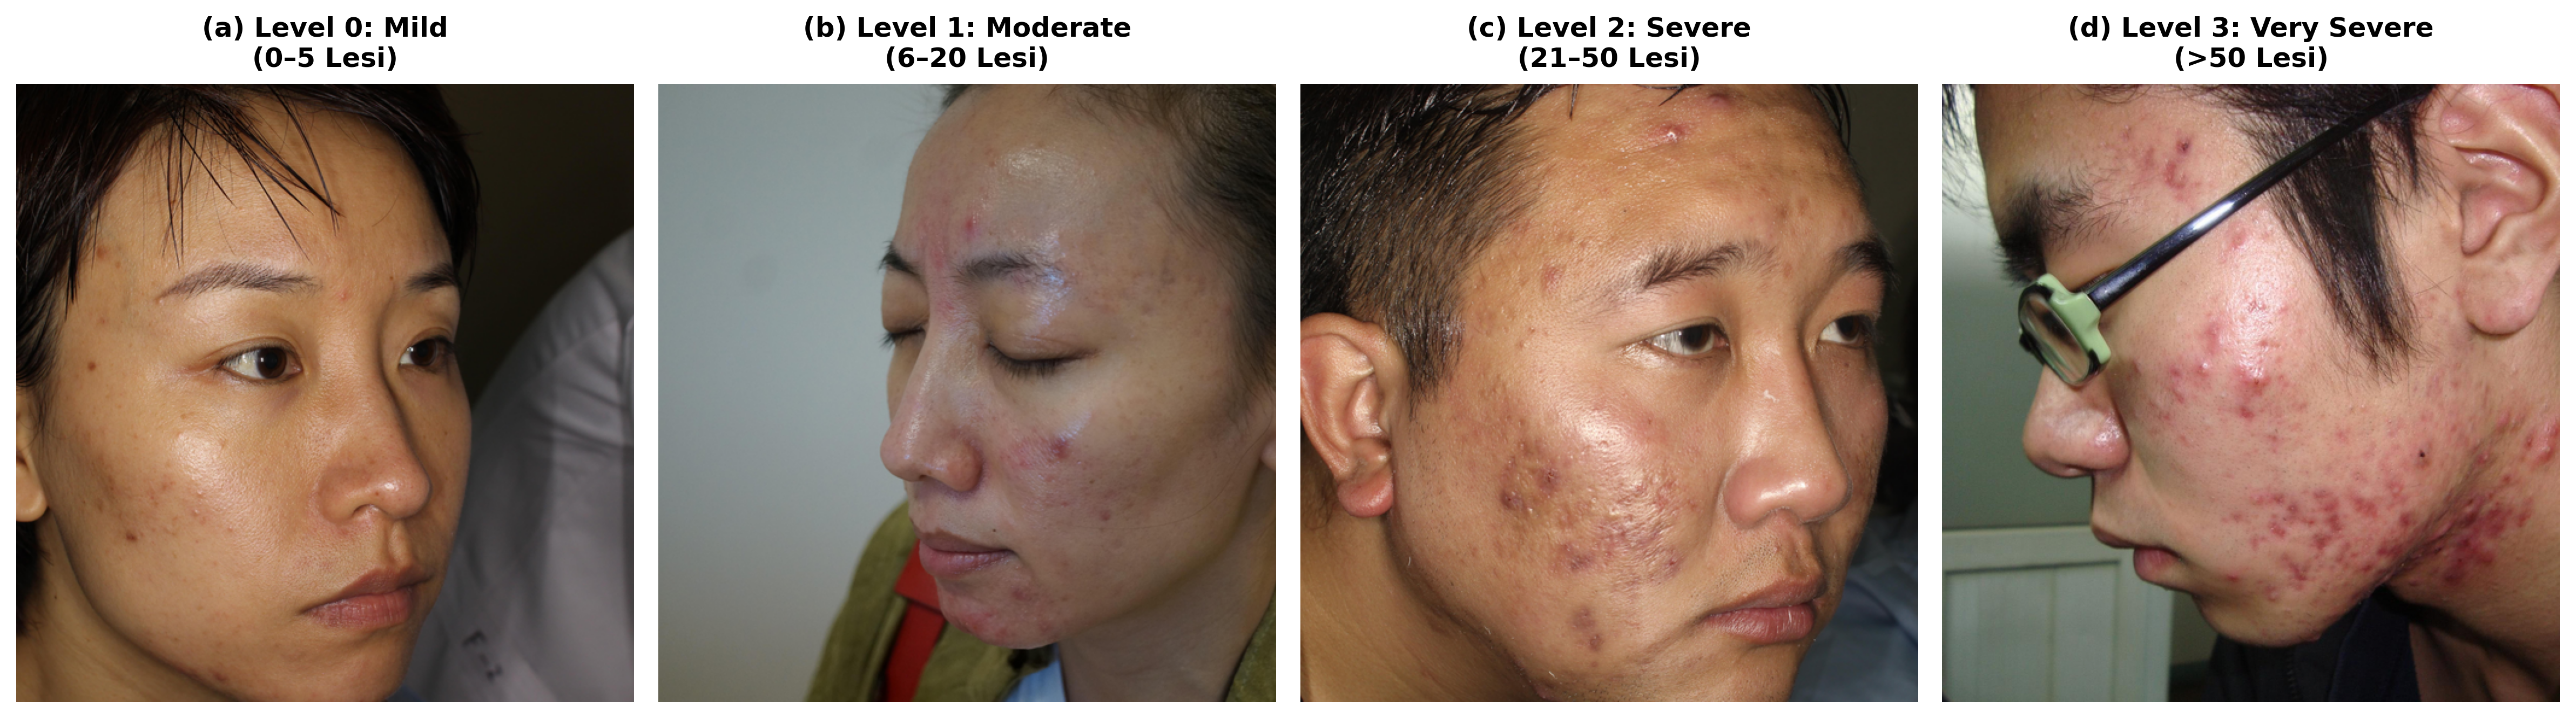
\includegraphics[width=\textwidth]{Gambar/acne04_collage_1x4_id.png}
    \caption{Sampel Citra Representatif Keempat Kelas Keparahan Jerawat (Level 0--3) pada Dataset \texttt{Layered-Labs/ACNE04} Berdasarkan Kriteria Hayashi.}
    \label{fig:acne04_collage}
\end{figure}

\subsection{\textit{Exploratory Data Analysis} (EDA)}
\label{subsec:eda_acne04}

Untuk memperoleh pemahaman empiris mengenai karakteristik fisik, struktur statistik, dan variabilitas visual dataset ACNE04 ($N = 1.457$), dilakukan prosedur \textit{Exploratory Data Analysis} (EDA) secara otomatis sebelum perancangan model.

\subsubsection{\textit{Class Distribution} dan \textit{Class Imbalance}}
Hasil audit empiris terhadap dataset \texttt{Layered-Labs/ACNE04} mengonfirmasi adanya \textit{class imbalance} yang substansial antarkelas. Distribusi kuantitatif dan proporsi relatif keempat kelas disajikan pada Gambar~\ref{fig:eda_class_distribution}.

\begin{figure}[!htbp]
    \centering
    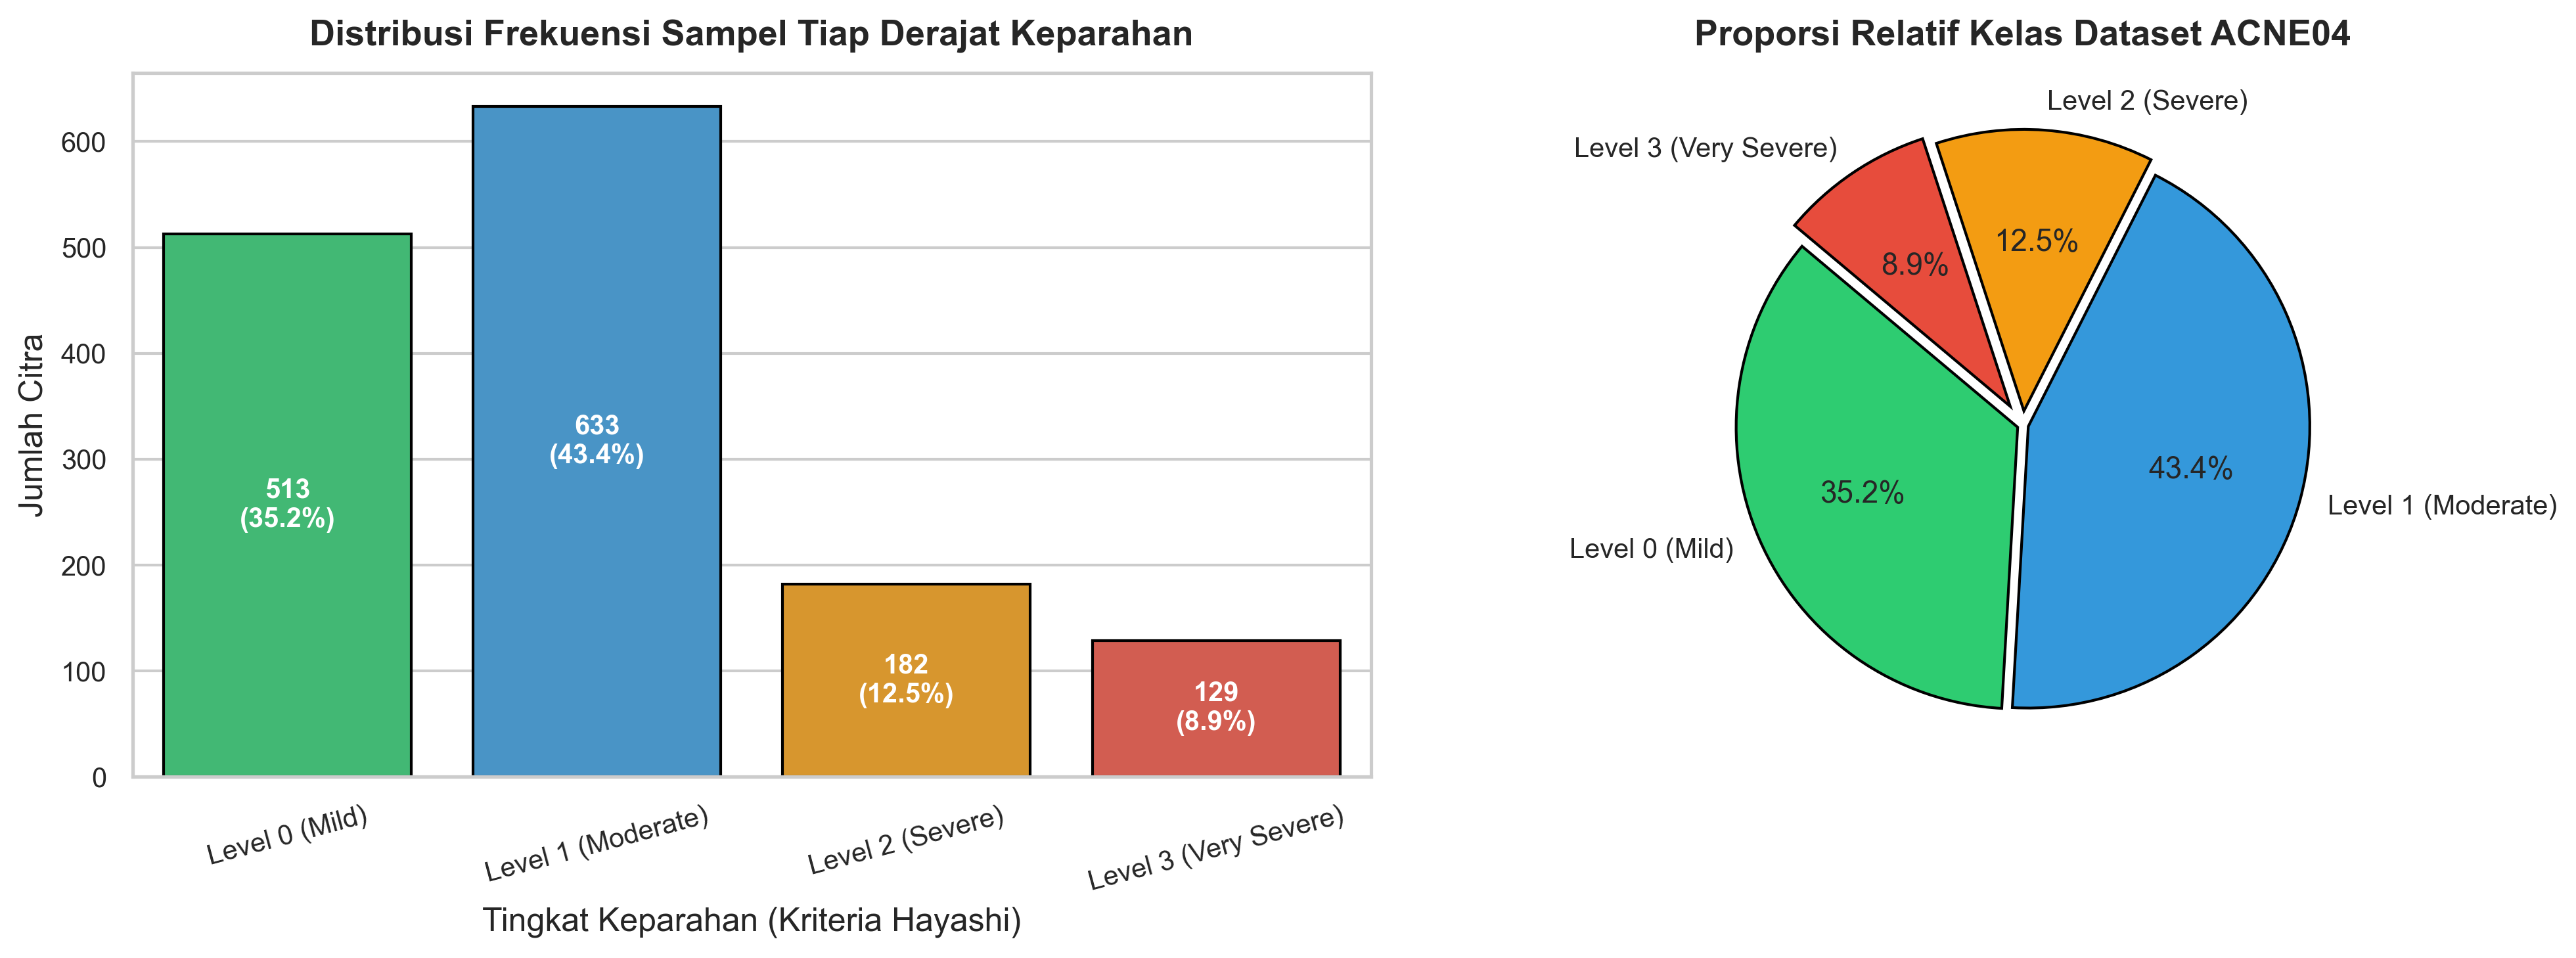
\includegraphics[width=0.92\textwidth]{Gambar/eda_class_distribution.png}
    \caption{Distribusi Frekuensi Sampel dan Proporsi Relatif Kelas pada Dataset ACNE04.}
    \label{fig:eda_class_distribution}
\end{figure}

Berdasarkan Gambar~\ref{fig:eda_class_distribution}, kelas mayoritas terkonsentrasi pada Level 1 (\textit{Moderate}) sebanyak $633$ citra ($43,45\%$) dan Level 0 (\textit{Mild}) sebanyak $513$ citra ($35,21\%$). Sebaliknya, kelas dengan tingkat keparahan tinggi memiliki jumlah sampel jauh lebih sedikit, yaitu Level 2 (\textit{Severe}) sebanyak $182$ citra ($12,49\%$) dan Level 3 (\textit{Very Severe}) sebanyak $129$ citra ($8,85\%$). Rasio \textit{class imbalance} antara kelas terbanyak (Level 1) dan kelas tersedikit (Level 3) mencapai $4,91 : 1,0$. Ketimpangan distribusi ini menjadi tantangan kritis karena fungsi \textit{cross-entropy} standar cenderung bias ke kelas mayoritas dan menurunkan sensitivitas terhadap kasus parah \cite{vut2025, zeng2026}, sehingga mendasari penggunaan \textit{weighted loss} serta metrik \textit{Macro F1-Score}, QWK, dan \textit{Class 3 Recall}.

\subsubsection{Karakteristik Dimensi Spasial dan \textit{File Size}}
Pemeriksaan dimensi geometris terhadap korpus \texttt{Layered-Labs/\allowbreak ACNE04} menunjukkan keberadaan $155$ resolusi spasial unik yang heterogen dengan lebar berkisar antara $143$ hingga $5.184$ piksel (median $3.112$ piksel), tinggi antara $155$ hingga $3.456$ piksel (median $3.456$ piksel), serta rasio aspek berkisar $0,562$--$1,778$ (median $0,900$). Sementara itu, ukuran berkas terkompresi memiliki median $855,49\text{ KB}$ (rentang interkuartil $679,99$--$962,80\text{ KB}$; minimum $3,25\text{ KB}$ dan maksimum $1.353,24\text{ KB}$). Heterogenitas resolusi dan komposisi latar belakang tersebut memvalidasi urgensi tahapan \textit{face cropping} dan standarisasi spasial menjadi $224\times224$ piksel sebelum pemrosesan \textit{Vision Transformer}.

\subsubsection{Profil Eritema (\textit{Erythema Index}) dan \textit{Color Space}}
Manifestasi peradangan jerawat secara visual dicirikan oleh eritema (kemerahan kulit akibat vasodilatasi vaskular). Untuk mengkuantifikasi kromatisitas ini pada sampel berimbang ($100$ citra per kelas), diekstraksi intensitas kanal Merah ($R$) RGB dan kanal $a^*$ dalam \textit{color space} perseptual CIE-LAB (sumbu hijau--merah), sebagaimana ditampilkan pada Gambar~\ref{fig:eda_erythema}.

\begin{figure}[!htbp]
    \centering
    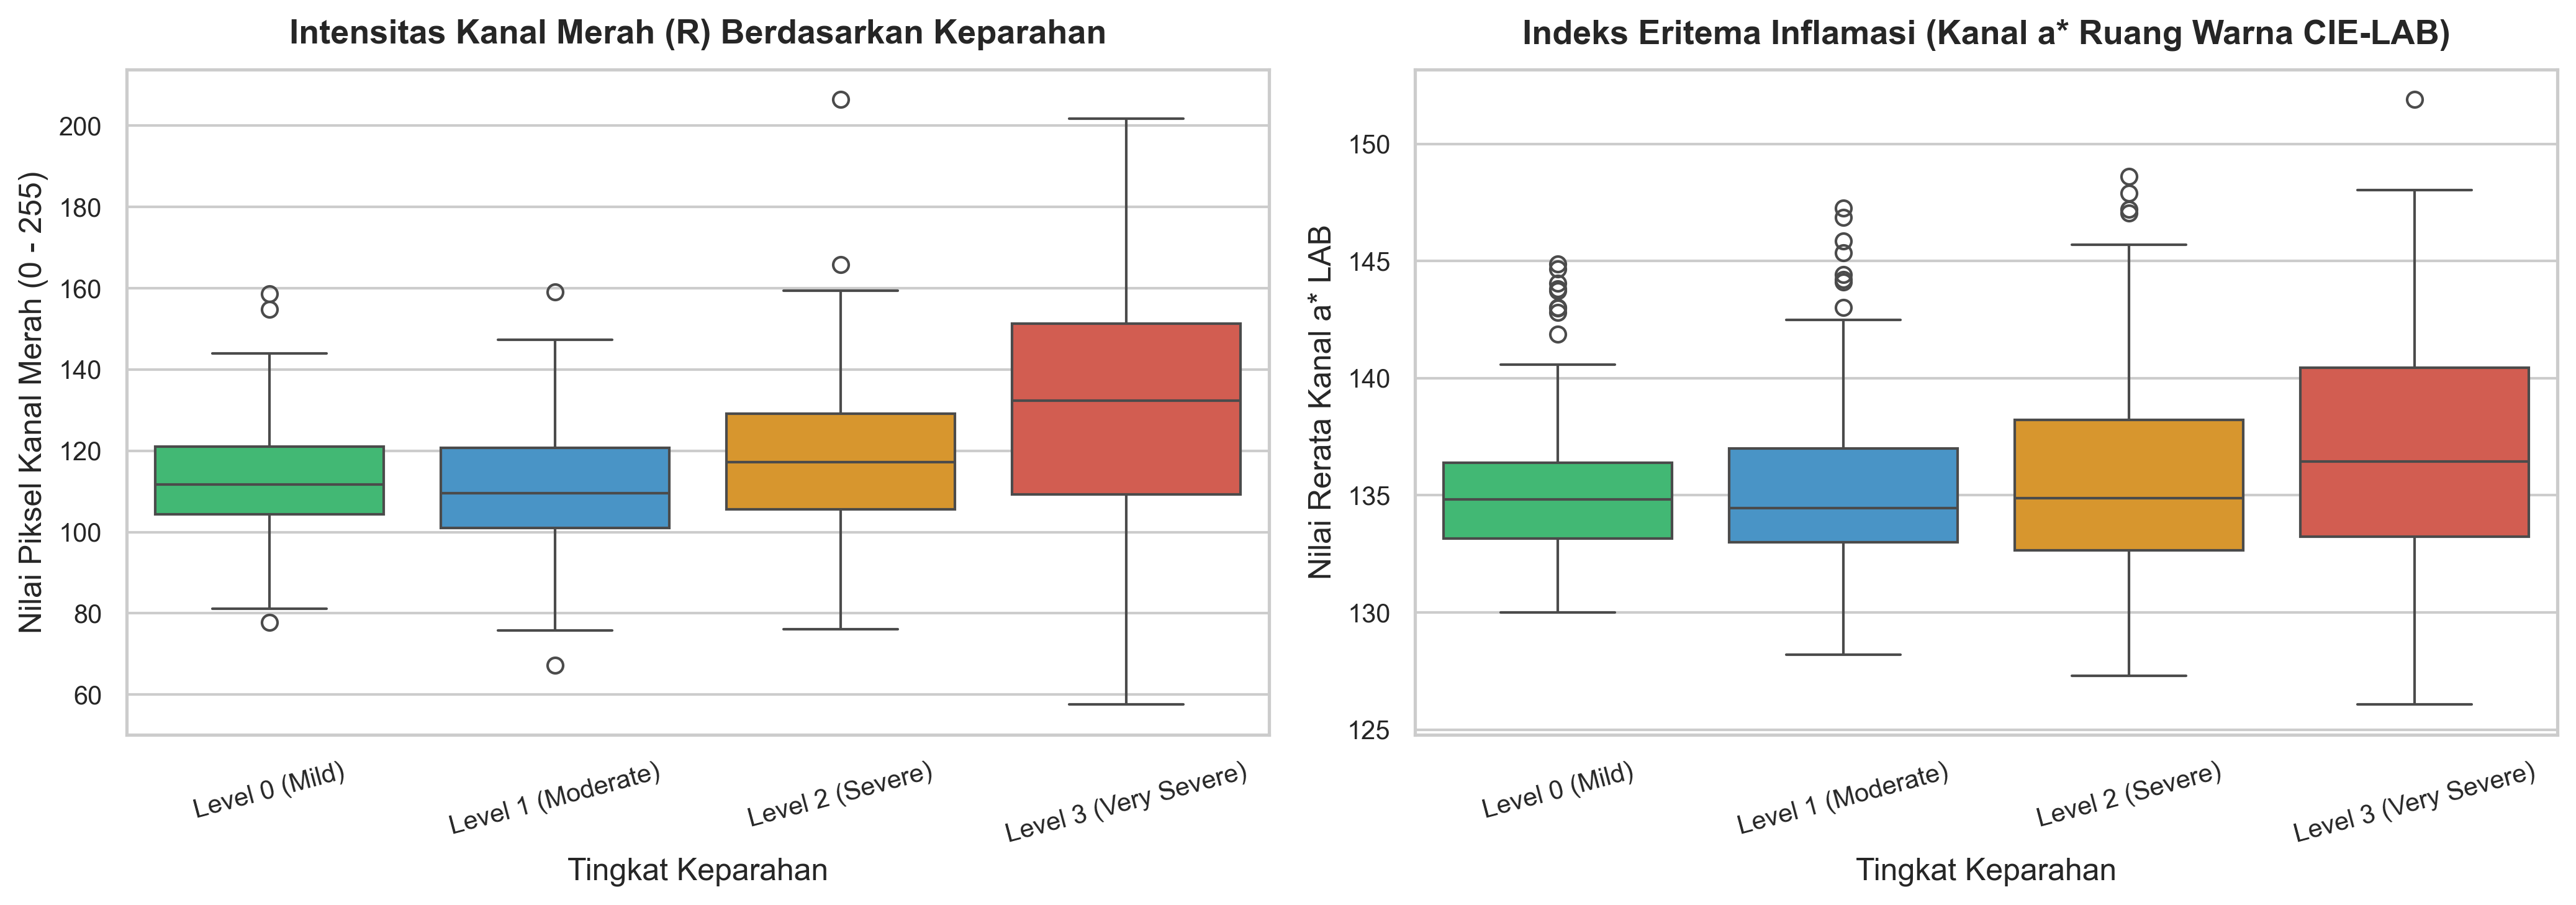
\includegraphics[width=0.92\textwidth]{Gambar/eda_erythema_analysis.png}
    \caption{Profil Distribusi Intensitas Kanal Merah dan Indeks Eritema (Kanal $a^*$ CIE-LAB) Berdasarkan Tingkat Keparahan Jerawat.}
    \label{fig:eda_erythema}
\end{figure}

Gambar~\ref{fig:eda_erythema} memperlihatkan kecenderungan peningkatan indeks kemerahan pada kanal $a^*$ CIE-LAB seiring naiknya tingkat keparahan, yakni dari rerata $135,43$ ($\sigma = 3,20$; median $134,82$) pada Level 0 menuju rerata $137,23$ ($\sigma = 5,53$; median $136,46$) pada Level 3 (\textit{Very Severe}). Tumpang tindih sebaran antar-kelas akibat perbedaan temperatur pencahayaan pemotretan memperkuat alasan penerapan \textit{color constancy} (\textit{Gray World}) serta penajaman kontras lokal (CLAHE).

\subsubsection{Normalisasi Empiris Dataset vs. Konstanta ImageNet}
Perhitungan statistik piksel global di seluruh $1.457$ citra \texttt{Layered-Labs/\allowbreak ACNE04} menghasilkan rerata RGB empiris $\mu = [0,4582;\allowbreak\; 0,3612;\allowbreak\; 0,2935]$ dan standar deviasi $\sigma = [0,2681;\allowbreak\; 0,2134;\allowbreak\; 0,1820]$. Dibandingkan dengan konstanta ImageNet ($\mu = [0,485;\; 0,456;\; 0,406]$ dan $\sigma = [0,229;\; 0,224;\; 0,225]$), terlihat pergeseran intensitas yang dominan ke spektrum \textit{warm skin tones}. Disparitas tersebut menegaskan adanya \textit{domain shift} antara citra objek alamiah dan fotografi dermatologi klinis sehingga menuntut \textit{fine-tuning} bobot DINOv3 secara teratur.

\subsection{\textit{Stratified Data Splitting}}
Untuk mencegah \textit{data leakage} sekaligus mempertahankan komposisi keempat kelas ordinal di setiap subset, $1.457$ citra dibagi menggunakan \textit{stratified split} 70:15:15 dengan perincian sebagai berikut:
\begin{itemize}
    \item \textbf{\textit{Train Set} (70\%):} $1.019$ citra (Level 0: $359$; Level 1: $443$; Level 2: $127$; Level 3: $90$), digunakan untuk pembaruan bobot model.
    \item \textbf{\textit{Validation Set} (15\%):} $219$ citra (Level 0: $77$; Level 1: $95$; Level 2: $27$; Level 3: $20$), digunakan untuk pemantauan \textit{validation loss}, \textit{learning rate scheduler}, dan pemilihan \textit{best checkpoints}.
    \item \textbf{\textit{Test Set} (15\%):} $219$ citra (Level 0: $77$; Level 1: $95$; Level 2: $28$; Level 3: $19$), dijaga terisolasi penuh untuk evaluasi akhir.
\end{itemize}

% -----------------------------------------------------------------------------
\section{\textit{Unified Single-Stream Preprocessing Pipeline}}
\label{sec:pipa_praproses}

Untuk menjamin konsistensi masukan antar-arsitektur pembanding, penelitian ini menerapkan \textit{unified single-stream preprocessing pipeline}. Seluruh citra melewati tahapan pembersihan latar belakang non-kulit, kalibrasi temperatur warna, peningkatan kontras lesi, isolasi area kulit wajah, standarisasi tensor, serta augmentasi klinis khusus \textit{Train Set} sebagaimana dirangkum pada Tabel~\ref{tab:tahap_preprocessing}. Ilustrasi visual perbandingan citra sebelum pemrosesan (\textit{before}), sesudah \textit{preprocessing} deterministik, dan sesudah augmentasi data disajikan pada Gambar~\ref{fig:before_after_preprocessing}.

\begin{table}[!htbp]
    \centering
    \caption{Tahapan \textit{Preprocessing} Satu Jalur dan Penanganan \textit{Class Imbalance}.}
    \label{tab:tahap_preprocessing}
    \footnotesize
    \renewcommand{\arraystretch}{1.25}
    \begin{tabularx}{\textwidth}{c >{\raggedright\arraybackslash}p{3.0cm} >{\raggedright\arraybackslash}X >{\raggedright\arraybackslash}X}
        \toprule
        \textbf{No} & \textbf{Komponen \textit{Pipeline}} & \textbf{Metode Operasional}                                                                                                      & \textbf{Deskripsi}                                                                                                               \\
        \midrule
        1           & \textit{Face Cropping}         & Deteksi wajah otomatis berbasis Haar Cascade dengan \textit{margin padding} 15\%                                         & Mengeliminasi latar belakang non-kulit (rambut, kerah pakaian, dinding) yang berpotensi memicu \textit{spurious features}.       \\
        \midrule
        2           & \textit{Skin Masking}          & Segmentasi area kulit lembut (\textit{soft skin mask}, $\alpha = 0,15$) melalui fusi \textit{color space} HSV dan YCbCr                             & Mereduksi intensitas wilayah non-epidermal sebesar 85\% agar representasi atensi berfokus pada permukaan kulit wajah.            \\
        \midrule
        3           & \textit{Color Constancy}       & Normalisasi \textit{white balance} menggunakan algoritma \textit{Gray World}                                                         & Menetralkan penyimpangan temperatur warna yang disebabkan sensor kamera dan pencahayaan ruangan heterogen.                       \\
        \midrule
        4           & \textit{CLAHE}                 & \textit{Contrast Limited Adaptive Histogram Equalization} ($clip=2,0$, \textit{grid} $8\times8$) pada kanal Luminansi ($L$) CIE-LAB          & Mempertajam visibilitas struktur mikrolesi (komedo, papula, pustula) tanpa merusak rona warna alami kulit.                      \\
        \midrule
        5           & \textit{Resize \& Normalize}   & Penyesuaian resolusi spasial $224\times224$ piksel dan normalisasi tensor RGB                                                    & Menyeragamkan dimensi tensor masukan agar terpartisi presisi menjadi 196 \textit{patches} berukuran $16\times16$ pada \textit{Vision Transformer}. \\
        \midrule
        6           & \textit{Data Augmentation} (\textit{Train Only}) & \textit{Random Horizontal Flip} ($p=0,5$), \textit{Safe Random Rotation} ($\pm15^\circ$), dan \textit{mild ColorJitter} ($\pm10\%$) & Menambah keragaman pose dan pencahayaan wajar tanpa mengubah jumlah maupun karakter patologis lesi kulit.                        \\
        \midrule
        7           & \textit{Cost-Sensitive Weight} & Pembobotan \textit{loss function} \textit{Weighted Cross-Entropy} berbasis frekuensi invers kelas                                & Mengatasi bias mayoritas dan mempertahankan sensitivitas deteksi terhadap kasus minoritas parah (Level 3).                       \\
        \bottomrule
    \end{tabularx}
\end{table}

\begin{figure}[!htbp]
    \centering
    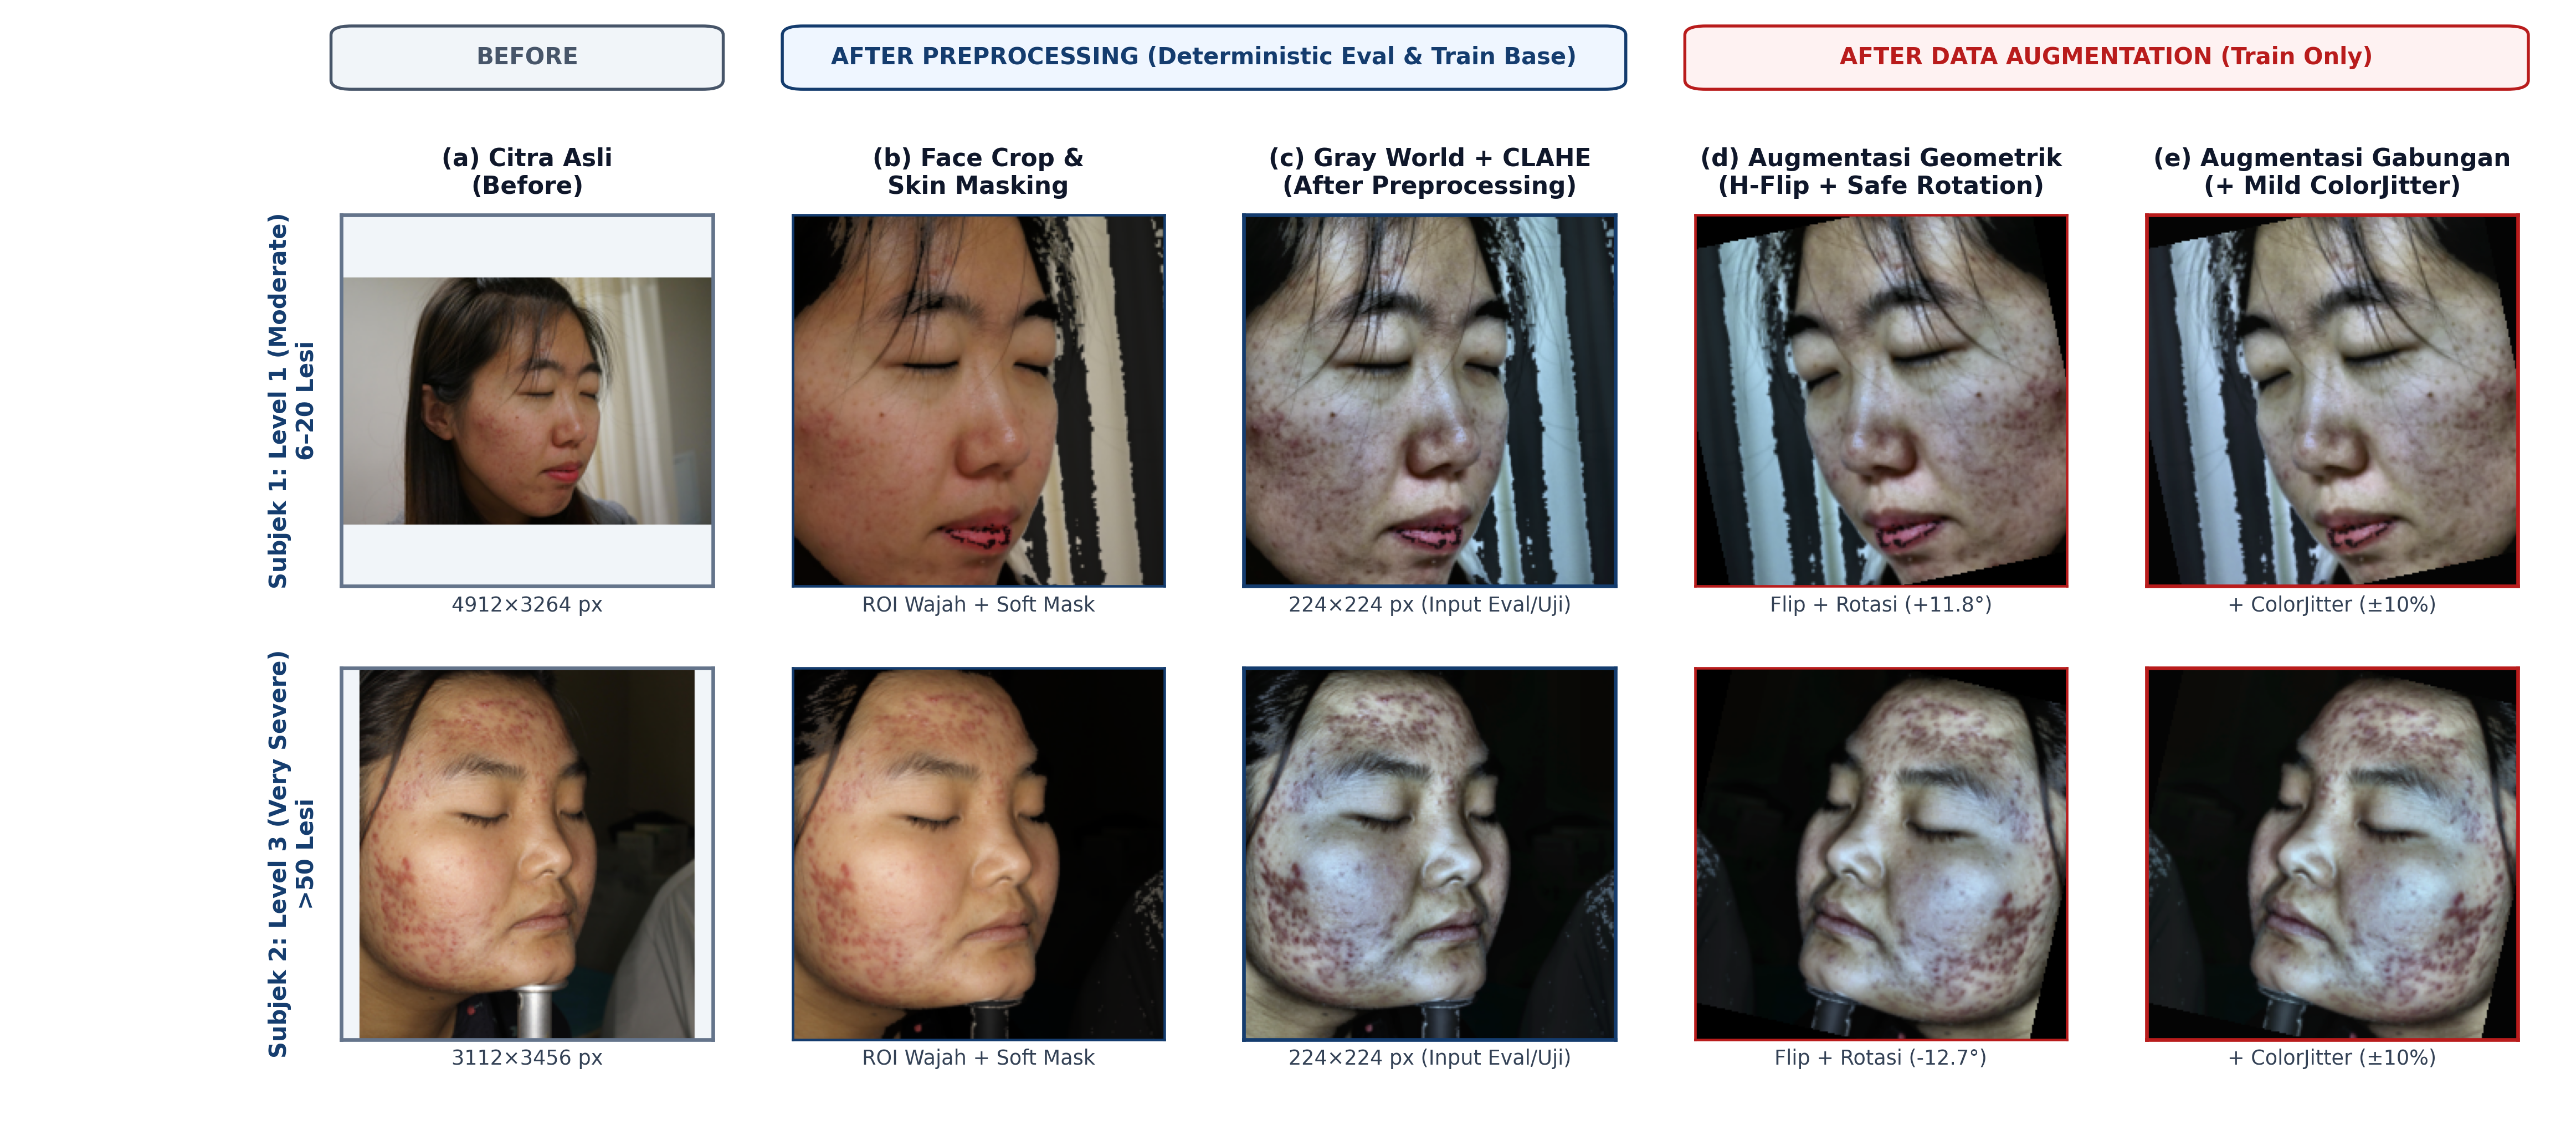
\includegraphics[width=\textwidth]{Gambar/preprocessing_augmentation_before_after.png}
    \caption{Perbandingan Visual Citra Sampel ACNE04 (Level 1 dan Level 3) pada kondisi awal (\textit{Before}), Sesudah \textit{Preprocessing} ($224\times224$ Piksel), dan Sesudah Augmentasi Data Klinis.}
    \label{fig:before_after_preprocessing}
\end{figure}

Secara khusus, pemilihan teknik \textit{data augmentation} hanya diterapkan pada \textit{Train Set} dengan batasan klinis yang masuk akal secara \textit{label-preserving}. Ketiga transformasi augmentasi yang dipilih beserta justifikasinya adalah:
\begin{itemize}
    \item \textbf{\textit{Random Horizontal Flip} ($p=0,5$):} Wajah manusia bersifat simetris secara bilateral; pencerminan horizontal kiri--kanan menyimulasikan variasi sudut pengambilan wajah tanpa mengubah jumlah total maupun klasifikasi tingkat keparahan lesi inflamasi.
    \item \textbf{\textit{Safe Random Rotation} ($\pm 15^\circ$):} Mengakomodasi variasi kemiringan posisi kepala pasien yang realistis saat pemeriksaan foto klinis. Sebaliknya, rotasi ekstrem maupun \textit{vertical flip} dihindari karena tidak realistis secara anatomis.
    \item \textbf{\textit{Mild ColorJitter} (\textit{brightness}, \textit{contrast}, \textit{saturation} $\pm 0,10$; \textit{hue} $\pm 0,03$):} Memperkaya variasi kecerahan dan kontras ruangan secara terukur; pergeseran \textit{hue} dibatasi ketat maksimal $\pm 0,03$ agar tidak mengubah eritema kemerahan secara artifisial. Transformasi destruktif seperti \textit{random erasing/cutout} juga dihindari karena berisiko menutupi kelompok pustula dan mengubah kelas label.
\end{itemize}

\subsection{Formulasi Matematis \textit{Preprocessing} dan \textit{Loss Weighting}}

\subsubsection{\textit{Contrast Limited Adaptive Histogram Equalization} (CLAHE)}
CLAHE diterapkan pada kanal luminansi ($L$) dari \textit{color space} CIE-LAB untuk mencegah amplifikasi \textit{noise} pada area homogen kulit \cite{wang2023}. Citra dibagi menjadi kisi blok kontekstual berukuran $8\times8$ piksel dengan pembatasan kontras (\textit{clipping limit} $= 2,0$), lalu kelebihan piksel didistribusikan merata sebelum interpolasi bilinear.

\subsubsection{\textit{Color Constancy} (\textit{Gray World})}
Variasi temperatur warna dinetralkan menggunakan algoritma \textit{Gray World}, yang mengasumsikan rerata reflektansi ketiga kanal warna mencerminkan abu-abu netral:
\begin{equation}
    k_c = \frac{1}{|I|} \sum_{x,y} I_c(x,y), \quad c \in \{R, G, B\}
\end{equation}
Setiap kanal diskalakan terhadap rata-rata global $\mu = \frac{k_R + k_G + k_B}{3}$ sehingga $I'_c(x,y) = I_c(x,y) \times \frac{\mu}{k_c}$.

\subsubsection{\textit{Cost-Sensitive Loss Weighting}}
Untuk mengompensasi rasio ketimpangan $4,91 : 1,0$, diterapkan bobot penalti frekuensi invers pada \textit{loss function} untuk setiap kelas $c \in \{0, 1, 2, 3\}$:
\begin{equation}
    w_c = \frac{N_{\text{train}}}{K \cdot N_c}
\end{equation}
dengan $N_{\text{train}} = 1.019$ adalah jumlah total sampel \textit{Train Set}, $K = 4$ jumlah kelas, dan $N_c$ jumlah sampel kelas $c$. Dengan formulasi ini, kelas minoritas Level 3 (\textit{Very Severe}, $N_3 = 90$) memperoleh bobot penalti tertinggi sehingga kesalahan prediksi pada kelas parah ditekan lebih kuat selama \textit{backpropagation}.

% -----------------------------------------------------------------------------
\section{Desain Arsitektur Model \textit{Transfer Learning}}
\label{sec:perancangan_arsitektur}

Penelitian ini mengadaptasi serta membandingkan dua skala arsitektur \textit{Vision Transformer} (ViT) dari keluarga \textit{vision foundation model} \textit{self-supervised} DINOv3 \cite{simeoni2025dinov3}. Rincian topologi blok encoder, \textit{register tokens}, dan perbandingan spesifikasi keduanya telah dipaparkan secara utuh pada Gambar~\ref{fig:arsitektur_dinov3} dan Tabel~\ref{tab:spesifikasi_dinov3} di Bab~II, yakni \textbf{DINOv3 ViT-L/16} (\textit{heavyweight}: 24 blok, $d=1.024$, 16 \textit{attention heads}, $\approx 304\text{M}$ parameter) serta \textbf{DINOv3 ViT-S/16} (\textit{lightweight}: 12 blok, $d=384$, 6 \textit{attention heads}, $\approx 21,6\text{M}$ parameter).

\subsection{\textit{Architecture Flow} dan \textit{Classification Head}}
Kedua model diinisialisasi menggunakan \textit{pre-trained weights} resmi DINOv3 \cite{simeoni2025dinov3} dan mengikuti aliran arsitektur terpadu dari tahap tokenisasi hingga klasifikasi ordinal. Citra wajah ter-preprocess berdimensi $224 \times 224 \times 3$ terlebih dahulu melalui lapisan konvolusi \textit{patch embedding} berukuran $16 \times 16$ piksel (\textit{stride} 16), menghasilkan kisi $14 \times 14 = 196$ \textit{patch tokens} yang digabungkan bersama satu token global \texttt{[CLS]}, empat \textit{register tokens}, serta \textit{axial Rotary Position Embedding} (RoPE). Rangkaian token tersebut melewati $L$ blok \textit{Transformer Encoder} ($L=24$ untuk ViT-L/16; $L=12$ untuk ViT-S/16) guna memodelkan relasi spasial lintas-area wajah. Pada luaran blok terakhir, vektor representasi token global \texttt{[CLS]} diekstraksi sebagai ringkasan fitur wajah menyeluruh:
\begin{equation}
    \mathbf{v}_{\text{[CLS]}} \in \mathbb{R}^{d_{\text{in}}}
\end{equation}
di mana $d_{\text{in}} = 1.024$ untuk DINOv3 ViT-L/16 dan $d_{\text{in}} = 384$ untuk DINOv3 ViT-S/16.

Untuk memetakan vektor laten ke empat kelas keparahan jerawat ordinal (Level 0--3), dibangun lapisan \textit{Linear Classification Head} kustom dengan regularisasi \textit{Dropout}:
\begin{equation}
    \mathbf{v}_{\text{[CLS]}} \xrightarrow{\text{Dropout}(p=0,2)} \mathbf{v}' \xrightarrow{\text{Linear}(d_{\text{in}} \to 4)} \hat{\mathbf{z}} \in \mathbb{R}^4
\end{equation}
Vektor \textit{logits} $\hat{\mathbf{z}}$ kemudian dikonversi melalui fungsi aktivasi \textit{softmax} menjadi distribusi probabilitas empat kelas:
\begin{equation}
    \hat{y}_c = \frac{\exp(\hat{z}_c)}{\sum_{j=0}^{3} \exp(\hat{z}_j)}, \quad c \in \{0, 1, 2, 3\}
\end{equation}

% -----------------------------------------------------------------------------
\section{Skenario \textit{Training} dan Optimasi}
\label{sec:skenario_pelatihan}

Proses \textit{training} seluruh model dijalankan menggunakan protokol komputasi dan lingkungan terstandarisasi berbasis pustaka PyTorch. Konfigurasi \textit{hyperparameter} eksperimen dirangkum pada Tabel~\ref{tab:hiperparameter_pelatihan}.

\begin{table}[!htbp]
    \centering
    \caption{Konfigurasi \textit{Hyperparameter Training} Model \textit{Transfer Learning} DINOv3.}
    \label{tab:hiperparameter_pelatihan}
    \small
    \renewcommand{\arraystretch}{1.25}
    \begin{tabularx}{\textwidth}{l >{\raggedright\arraybackslash}X}
        \toprule
        \textbf{\textit{Hyperparameter}}               & \textbf{Nilai / Konfigurasi}                                                             \\
        \midrule
        Arsitektur Model                               & DINOv3 ViT-L/16 (\textit{Heavyweight}) dan DINOv3 ViT-S/16 (\textit{Lightweight})        \\
        \textit{Input Dimension}                       & $224 \times 224 \times 3$ piksel ($196$ \textit{patch tokens} berukuran $16\times16$)     \\
        \textit{Batch Size}                            & $16$                                                                                     \\
        \textit{Optimizer}                             & AdamW (\textit{weight decay} $= 1\times 10^{-4}$)                                        \\
        \textit{Initial Learning Rate} ($\eta_0$)      & $1\times 10^{-4}$ (ViT-S/16) dan $5\times 10^{-5}$ (ViT-L/16)                            \\
        \textit{Learning Rate Scheduler}               & \textit{Cosine Annealing} ($T_{\text{max}} = 50$, $\eta_{\text{min}} = 1\times 10^{-6}$) \\
        \textit{Loss Function}                         & \textit{Weighted Categorical Cross-Entropy Loss}                                         \\
        Maksimum \textit{Epoch}                        & $50$ \textit{epoch}                                                                      \\
        \textit{Early Stopping}                        & \textit{Patience} $= 10$ \textit{epoch} pada metrik \textit{Validation Macro-F1}         \\
        Perangkat Keras                                & NVIDIA GPU dengan akselerasi CUDA                                                        \\
        \bottomrule
    \end{tabularx}
\end{table}

\subsection{\textit{Input Dimension} dan \textit{Batch Size}}
Dimensi spasial citra masukan ditetapkan sebesar $224 \times 224 \times 3$ piksel sehingga citra terpartisi presisi menjadi kisi $14 \times 14$ ($196$ \textit{patch tokens}) berukuran $16 \times 16$ piksel tanpa distorsi interpolasi. Resolusi ini menjaga ketajaman tekstur mikrolesi jerawat sekaligus menstabilkan kebutuhan memori VRAM GPU \cite{simeoni2025dinov3}.

Nilai \textit{batch size} ditetapkan sebesar $16$ sampel per iterasi guna mengakomodasi graf komputasi DINOv3 ViT-L/16 ($\approx 304\text{M}$ parameter) pada satu GPU serta memberikan regularisasi gradien stokastik pada \textit{Train Set} ($N_{\text{train}} = 1.019$) \cite{davila2024}.

\subsection{\textit{Optimizer} dan \textit{Weight Decay}}
Optimasi parameter menggunakan \textit{optimizer} AdamW (\textit{decoupled weight decay}) dengan koefisien \textit{weight decay} $= 1 \times 10^{-4}$. Pada arsitektur \textit{Vision Transformer}, pemisahan \textit{weight decay} dari estimasi momen adaptif mencegah distorsi skala gradien sehingga meminimalkan risiko \textit{catastrophic forgetting} terhadap representasi umum \textit{vision foundation model} DINOv3 \cite{simeoni2025dinov3}.

\subsection{\textit{Learning Rate} dan \textit{Cosine Annealing Scheduler}}
Nilai \textit{initial learning rate} ditetapkan $\eta_0 = 1 \times 10^{-4}$ untuk DINOv3 ViT-S/16 dan $\eta_0 = 5 \times 10^{-5}$ yang lebih konservatif untuk DINOv3 ViT-L/16 agar pembaruan bobot pada $24$ blok atensi tidak memicu osilasi gradien awal. Peluruhan \textit{learning rate} selama $50$ \textit{epoch} dikendalikan melalui \textit{Cosine Annealing Scheduler}:
\begin{equation}
    \eta_t = \eta_{\text{min}} + \frac{1}{2}(\eta_0 - \eta_{\text{min}})\left(1 + \cos\left(\frac{t}{T_{\text{max}}}\pi\right)\right)
\end{equation}
dengan $\eta_{\text{min}} = 1 \times 10^{-6}$ dan $T_{\text{max}} = 50$.

\subsection{\textit{Weighted Categorical Cross-Entropy Loss}}
Kondisi \textit{class imbalance} dataset \texttt{Layered-Labs/ACNE04} (rasio Level 1 terhadap Level 3 sebesar $4,91 : 1,0$) dimitigasi menggunakan \textit{loss function} \textit{Weighted Categorical Cross-Entropy} ($\mathcal{L}_{\text{WCE}}$):
\begin{equation}
    \mathcal{L}_{\text{WCE}} = - \frac{1}{B} \sum_{i=1}^{B} \sum_{c=0}^{3} w_c \cdot y_{i,c} \log(\hat{y}_{i,c})
\end{equation}
di mana $B = 16$ adalah \textit{batch size}, $y_{i,c} \in \{0, 1\}$ label \textit{one-hot}, $\hat{y}_{i,c}$ probabilitas \textit{softmax}, dan $w_c = \frac{N_{\text{train}}}{K \cdot N_c}$ bobot penalti kelas ($N_{\text{train}} = 1.019$, $K = 4$). Kesalahan klasifikasi pada kelas minoritas Level 3 dikenakan penalti gradien terbesar agar model membentuk batas keputusan yang seimbang di seluruh kelas \cite{vut2025}.

\subsection{\textit{Convergence Criteria} dan \textit{Early Stopping}}
Proses \textit{training} dijalankan hingga maksimum $50$ \textit{epoch} dengan mekanisme \textit{early stopping} (\textit{patience} $= 10$ \textit{epoch}) yang memantau \textit{Validation Macro-F1} guna mencegah \textit{overfitting}. Bobot model terbaik (\textit{best checkpoint}) dipilih untuk evaluasi akhir.

% -----------------------------------------------------------------------------
\section{Metrik Evaluasi Kinerja}
\label{sec:metrik_evaluasi}

Kinerja seluruh model diuji secara menyeluruh pada subset \textit{Test Set} independen yang terisolasi ($N_{\text{test}} = 219$; distribusi: Level 0 $= 77$, Level 1 $= 95$, Level 2 $= 28$, Level 3 $= 19$). Mengingat ketimpangan distribusi serta sifat ordinal tingkat keparahan jerawat, evaluasi mengombinasikan akurasi global, metrik \textit{macro-averaging}, kesepakatan ordinal \textit{Quadratic Weighted Kappa}, sensitivitas Level 3, dan \textit{confusion matrix} numerik \cite{davila2024, vut2025}.

\subsection{\textit{Accuracy}}
\textit{Accuracy} mengukur proporsi total prediksi tepat terhadap seluruh sampel uji ($N_{\text{test}} = 219$):
\begin{equation}
    \text{Accuracy} = \frac{\sum_{c=0}^{3} TP_c}{N_{\text{test}}}
\end{equation}
dengan $TP_c$ menyatakan jumlah \textit{True Positive} kelas ke-$c$.

\subsection{\textit{Macro Precision}}
\textit{Macro Precision} mengevaluasi ketepatan rata-rata prediksi positif secara merata di seluruh empat kelas (Level 0, Level 1, Level 2, dan Level 3):
\begin{equation}
    \text{Precision}_{\text{macro}} = \frac{1}{4} \sum_{c=0}^{3} \frac{TP_c}{TP_c + FP_c}
\end{equation}
di mana $FP_c$ adalah jumlah \textit{False Positive} kelas ke-$c$. Presisi yang tinggi pada seluruh kelas meminimalkan risiko \textit{over-diagnosis} yang dapat berujung pada intervensi klinis berlebih \cite{hayashi2008, lopez2023}.

\subsection{\textit{Macro Recall}}
\textit{Macro Recall} mengukur rata-rata kemampuan model menjaring kembali seluruh sampel aktual pada keempat kelas (Level 0, Level 1, Level 2, dan Level 3):
\begin{equation}
    \text{Recall}_{\text{macro}} = \frac{1}{4} \sum_{c=0}^{3} \frac{TP_c}{TP_c + FN_c}
\end{equation}
di mana $FN_c$ adalah jumlah \textit{False Negative} kelas ke-$c$, yang mencerminkan kemampuan pencegahan \textit{under-diagnosis} secara merata di seluruh kelas tanpa didominasi kelas mayoritas.

\subsection{\textit{Macro F1-Score}}
\textit{Macro F1-Score} menghitung rata-rata harmonik dari \textit{Precision} dan \textit{Recall} secara setara di seluruh empat kelas:
\begin{equation}
    \text{F1}_{\text{macro}} = \frac{1}{4}\sum_{c=0}^{3} \frac{2 \cdot \text{Precision}_c \cdot \text{Recall}_c}{\text{Precision}_c + \text{Recall}_c}
\end{equation}
Metrik ini dijadikan tolok ukur pemilih model terbaik karena memberi bobot identik $25\%$ pada setiap kelas \cite{davila2024, zeng2026}.

\subsection{\textit{Quadratic Weighted Kappa} (QWK)}
Karena kelas Level 0 hingga Level 3 bersifat ordinal berurutan, kesalahan klasifikasi sejauh tiga tingkat (misalnya Level 3 diprediksi sebagai Level 0) jauh lebih berbahaya secara klinis daripada pergeseran satu tingkat bertetangga. Oleh karena itu, digunakan \textit{Quadratic Weighted Kappa} (QWK, $\kappa_w$) yang mengukur tingkat kesesuaian prediksi terhadap label klinis dengan bobot penalti kuadratik atas jarak kesalahan kelas \cite{cohen1968weighted}:
\begin{equation}
    \kappa_w = 1 - \frac{\sum_{i=0}^{3}\sum_{j=0}^{3} w_{i,j}\, O_{i,j}}{\sum_{i=0}^{3}\sum_{j=0}^{3} w_{i,j}\, E_{i,j}}, \qquad w_{i,j} = \frac{(i - j)^2}{(K - 1)^2}
\end{equation}
di mana $K = 4$, $O_{i,j}$ adalah \textit{confusion matrix} pengamatan, $E_{i,j}$ matriks harapan peluang acak di bawah independensi marginal, dan $w_{i,j} \in [0, 1]$ bobot kuadratik ($w_{0,0}=0$, pergeseran $1$ tingkat $w_{i,i\pm1}=1/9$, sedangkan kesalahan ekstrem $w_{0,3}=1$). Nilai QWK berada pada rentang $[-1, 1]$: nilai $\le 0$ menandakan kesepakatan setara atau lebih buruk dari tebakan acak; nilai $0,01$--$0,40$ dinilai lemah--cukup; $0,41$--$0,60$ sedang (\textit{moderate}), $0,61$--$0,80$ substansial (\textit{substantial}), dan rentang $0,81$--$1,00$ dikategorikan hampir sempurna (\textit{almost perfect agreement}) dan layak untuk sistem penunjang diagnosis klinis \cite{landis1977measurement, zeng2026}.

\subsection{\textit{Class 3 Recall} dan \textit{Confusion Matrix}}
Kesalahan \textit{under-diagnosis} pada pasien Level 3 membawa konsekuensi klinis paling berat karena menunda terapi sistemik \cite{hayashi2008, vut2025}, sehingga sensitivitas kelas paling parah diukur secara khusus melalui:
\begin{equation}
    \text{Recall}_{3} = \frac{C_{3,3}}{\sum_{j=0}^{3} C_{3,j}}
\end{equation}
di mana $C_{i,j}$ merupakan sel pada \textit{confusion matrix} berukuran $4 \times 4$. Sesuai standar penomoran kelas pada Tabel~\ref{tab:distribusi_acne04}, seluruh label baris dan kolom pada \textit{confusion matrix} menggunakan notasi numerik murni (\texttt{0}, \texttt{1}, \texttt{2}, \texttt{3}) guna meringkas tampilan tanpa pengulangan teks kategori (0 = \textit{Mild}, 1 = \textit{Moderate}, 2 = \textit{Severe}, 3 = \textit{Very Severe}), sebagaimana diformat pada Tabel~\ref{tab:template_confusion_matrix}. Selain metrik kuantitatif penuh tersebut, kasus dengan selisih probabilitas top-1 dan top-2 yang sempit ($\Delta p < 0,15$) dicatat sebagai penanda \textit{borderline ambiguity} pada berkas log CSV untuk analisis galat kualitatif di sekitar batas kelas Hayashi.

\begin{table}[!htbp]
    \centering
    \caption{Struktur \textit{Confusion Matrix} Empat Kelas Bernotasi Numerik (\textit{Test Set}, $N_{\text{test}} = 219$).}
    \label{tab:template_confusion_matrix}
    \small
    \renewcommand{\arraystretch}{1.25}
    \begin{tabular}{c c cccc c}
        \toprule
        & & \multicolumn{4}{c}{\textbf{Prediksi Model (\textit{Predicted})}} & \\
        \cmidrule(lr){3-6}
        & & \textbf{0} & \textbf{1} & \textbf{2} & \textbf{3} & \textbf{Total} \\
        \midrule
        \multirow{4}{*}{\makecell{\textbf{Aktual}\\\textbf{(\textit{True})}}}
        & \textbf{0} & $C_{0,0}$ & $C_{0,1}$ & $C_{0,2}$ & $C_{0,3}$ & $77$ \\
        & \textbf{1} & $C_{1,0}$ & $C_{1,1}$ & $C_{1,2}$ & $C_{1,3}$ & $95$ \\
        & \textbf{2} & $C_{2,0}$ & $C_{2,1}$ & $C_{2,2}$ & $C_{2,3}$ & $28$ \\
        & \textbf{3} & $C_{3,0}$ & $C_{3,1}$ & $C_{3,2}$ & $C_{3,3}$ & $19$ \\
        \midrule
        \multicolumn{2}{c}{\textbf{Total}} & $\sum_i C_{i,0}$ & $\sum_i C_{i,1}$ & $\sum_i C_{i,2}$ & $\sum_i C_{i,3}$ & $\mathbf{219}$ \\
        \bottomrule
    \end{tabular}
\end{table}
